% Chapter Template

\chapter{Validació del sistema} % Main chapter title

Definits els components i detalls que componen el sistema de monitoratge i el sistema d'adaptabilitat, i un cop justificada des d'un punt de vista teòric la satisfacció dels nostres objectius, és el moment de presentar un exemple de cas d'ús i provar l'execució per validar el seu funcionament satisfactori i avaluar els resultats obtinguts.

\section{Presentació de cas d'ús}

Recordem la premissa genèrica del cas d'ús que volem que el nostre sistema satisfaci:

\begin{center}
\textit{Donada un \textbf{procés de monitoratge actiu} en un dels monitors del nostre sistema, i una proposta de \textbf{nova configuració} modelada, volem executar de forma automatitzada una \textbf{reconfiguració} d'aquell procés de monitoratge d'acord amb els \textbf{canvis computats respecte l'actual}.}
\end{center}

Per validar aquesta execució necessitem definir: un \textit{Base Model} que modeli l'estat actual del sistema (figura ~\ref{fig:Figura37}, una \textit{Feature Configuration} que modeli la darrera aplicada al sistema (figura ~\ref{fig:Figura37}, una \textit{Feature Configuration} que modeli la nova proposta de configuració del sistema (figura ~\ref{fig:Figura38}) i un \textit{Adaptability Model} que defineixi l'adaptació de models i la reconfiguració  de monitors (figura ~\ref{fig:Figura39}).\\

\begin{figure}
\centering
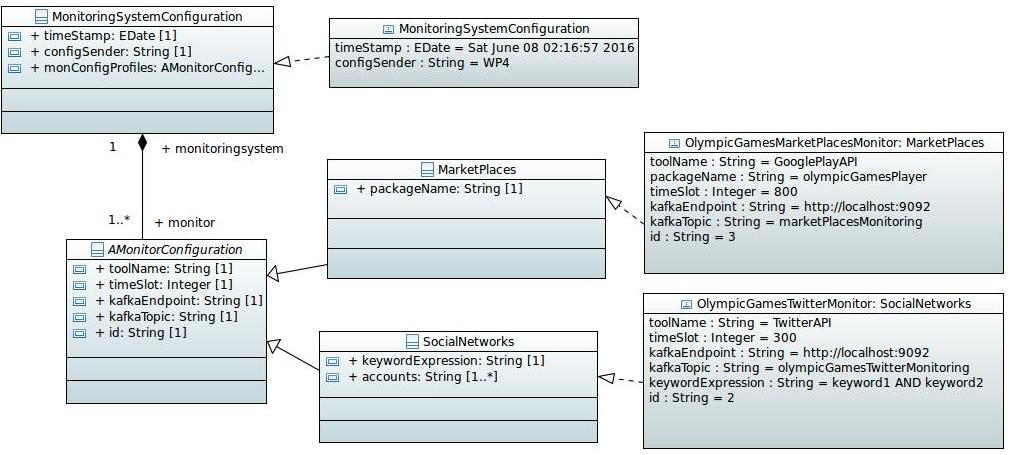
\includegraphics[width=14cm]{Figures/Figure16}
\decoRule
\caption{\textit{Base Model} utilitzat per validar la reconfiguració del sistema}
\label{fig:Figura36}
\end{figure} 

Com podem veure, el \textit{Base Model} defineix una configuració del sistema de monitoratge (ja vista anteriorment com a exemple en el \textit{Capítol 8. Modelatge UML de les configuracions de monitors}) amb dues instàncies de processos de monitoratge corrent: una sobre el monitor de Twitter, i l'altra sobre el monitor de Google Play, ambdues configurades amb els seus propis paràmetres de configuració. Pel nostre cas d'estudi, suposarem que aquest és el darrer \textit{Base Model} que defineix l'estat del sistema. Per la reconfiguració ens centrarem exclusivament en el procés de monitoratge de Twitter, el qual hem inicialitzat amb els paràmetres \textit{keywordExpression} i \textit{accounts} tal i com es mostra a la figura, per facilitar el \textit{testing}.\\

Si ens fixem en les dues \textit{Feature Configuration}, veiem que aquestes són pràcticament les mateixes, a excepció de l'atribut \textit{timeSlot} per les instàncies del monitor de Twitter que, en la nova proposta de configuració, pren un valor més elevat (de 30 segons passa a valer 50). S'ha triat aquest cas d'ús (la modificació del \textit{timeSlot}) per la validació del sistema per dos motius: primerament, per tractar-se d'un cas bàsic que permet observar amb detall la reconfiguració basant-nos en un únic punt de variabilitat, i segon perquè la modificació d'aquest \textit{timeSlot} serà fàcilment visualitzable en el procés d'execució dels monitors.\\ 

Finalment, l'\textit{Adaptability Model} descriu la \textit{feature} timeSlot com a \textit{feature} sobre la qual defineix una adaptació, així com els \textit{patterns} i rols a aplicar sobre els models, i finalment l'acció d'actualització del \textit{timeSlot} d'acord amb el valor definit.\\

\begin{figure}
\centering
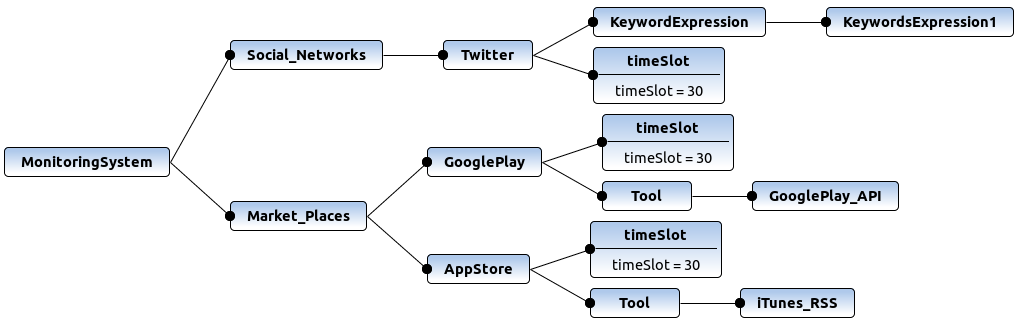
\includegraphics[width=14cm]{Figures/Figure36}
\decoRule
\caption{\textit{Feature Configuration} que descriu la darrera configuració del sistema aplicada}
\label{fig:Figura37}
\end{figure} 

\begin{figure}
\centering
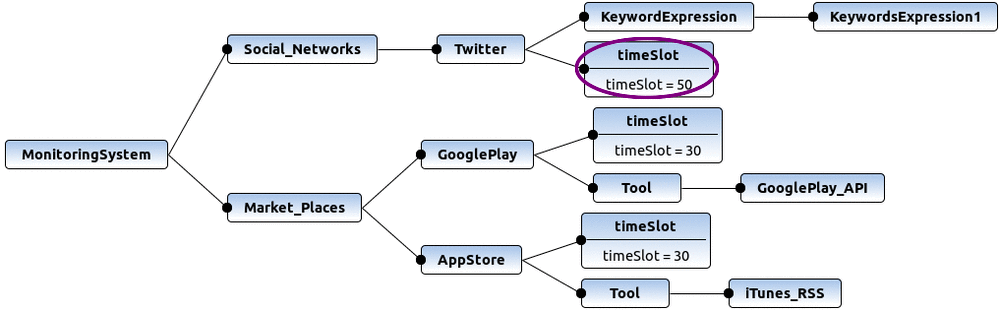
\includegraphics[width=14cm]{Figures/Figure37}
\decoRule
\caption{\textit{Feature Configuration} que descriu la configuració a aplicar per la reconfiguració}
\label{fig:Figura38}
\end{figure} 

\begin{figure}
\centering
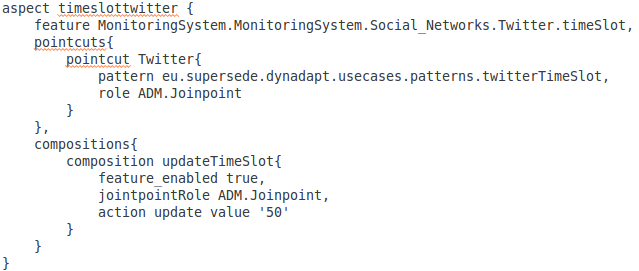
\includegraphics[width=14cm]{Figures/Figure38}
\decoRule
\caption{\textit{Adaptability Model} que descriu la reconfiguració a executar}
\label{fig:Figura39}
\end{figure} 

\section{Execució de la reconfiguració}

El disparador de l'execució serà la sol·licitud a través del \textit{dashboard} de la reconfiguració associada a la \textit{Feature Configuration} anomenada \textit{MonitoringSystemConfigHighTimeslot}. A la figura ~\ref{fig:dashboard1} podem visualitzar un exemple de visualització de la vista \textit{Suggested Adaptations}, que en aquest cas mostra una única \textit{Feature Configuratio} amb una sola acció: l'actualització del valor \textit{timeslot} de les instàncies del monitor de Twitter a 50 segons. Quan l'usuari fa click al botó \textit{"Enact"} amb la \textit{Feature Configuration} seleccionada, el \textit{Dashboard} construeix la sol·licitud amb les dades d'aquella nova configuració, i envia a l'Adapter la petició de reconfiguració. En aquest punt, s'executa l'algorisme de reconfiguració descrit al \textit{Capítol 9. Sistema d'adaptabilitat}, amb la única diferència que la \textit{Feature Configuration} ve donada per paràmetre d'entrada (utilitzem aquest mètode, descrit a la interfície de l'Adapter també present al mateix capítol, per facilitar la validació). Un cop l'Adapter finalitza la seva execució, obté una instància de l'Enactor, que a través dels models UML (l'original i l'adaptat) computa una petició a l'Orchestrator que representa l'actualització de la configuració amb els nous valors. A partir d'aquí, el \textit{workflow} de la reconfiguració passa a estar en mans del sistema de monitoratge. L'Orchestrator envia la petició al Monitor Manager, i aquest la deriva al monitor corresponent. En aquest cas, corresponent al monitor de Twitter.\\

\begin{figure}[H]
\centering
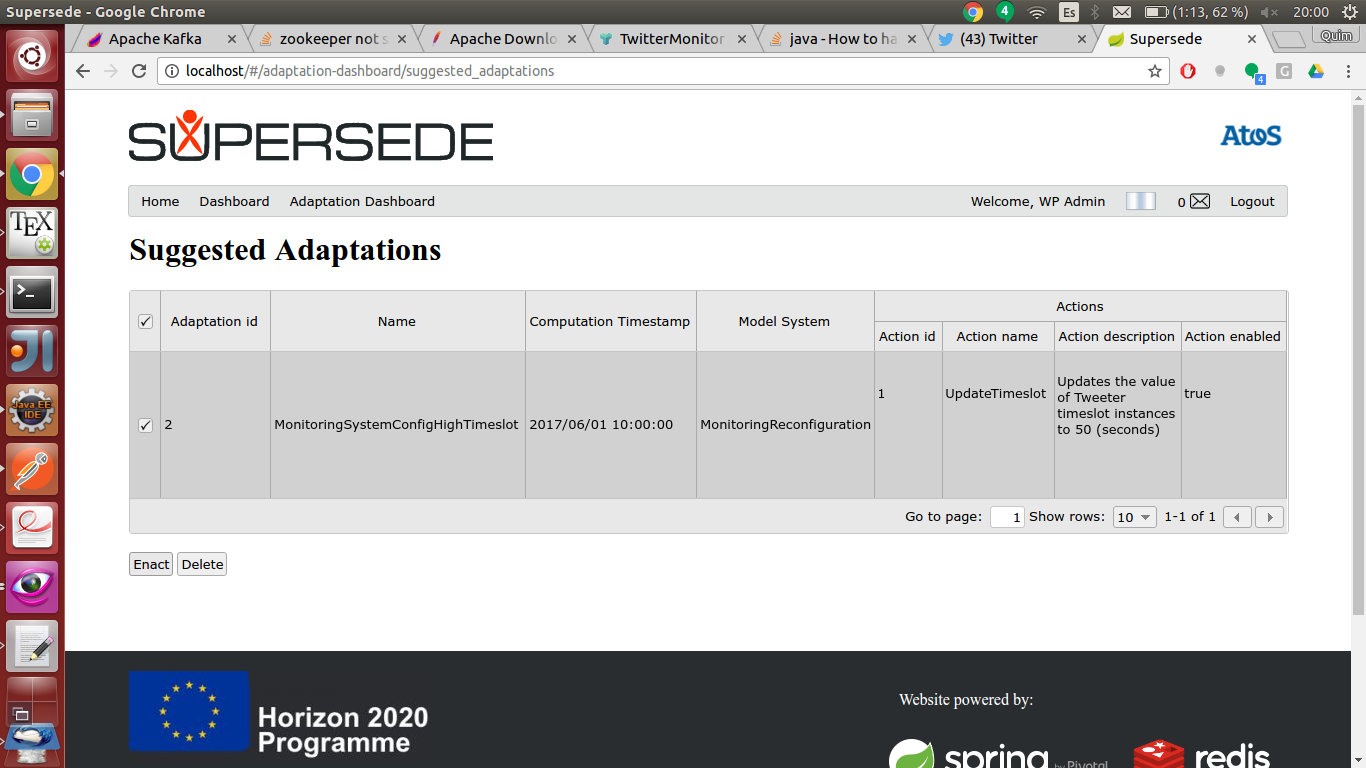
\includegraphics[width=14cm]{Figures/dashboard1}
\decoRule
\caption{Sol·licitud d'execució de l'adaptació \textit{MonitoringSystemConfigHighTimeslot}}
\label{fig:dashboard1}
\end{figure} 

\begin{figure}[H]
\centering
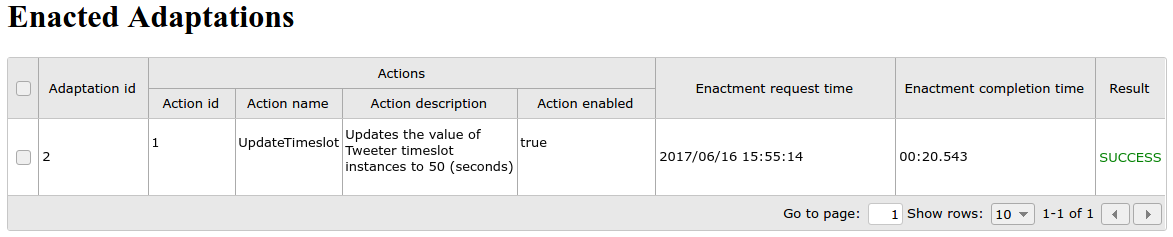
\includegraphics[width=14cm]{Figures/dashboard2}
\decoRule
\caption{Resultats de l'execució de l'adaptació \textit{MonitoringSystemConfigHighTimeslot}}
\label{fig:dashboard2}
\end{figure} 

Cal recordar que tota la comunicació de components es realitza a través de IF (a excepció d'alguns components que es despleguen de forma integrada ja que actuen com a auxiliars, com és el cas del Model Adapter i l'Enactor respecte l'Adapter). Per tant, serà aquest el responsable de rebre i redireccionar les peticions, i conèixer en cada cas on es troben desplegats cadascun dels components amb els quals s'ha d'enviar la petició.\\

Un cop finalitzada aquesta reconfiguració, des del punt de vista del sistema d'adaptabilitat podem consultar la modificació des de la perspectiva teòrica. Si consultem la vista d'adaptacions executades, mostrada a la figura ~\ref{fig:dashboard2}, podem veure com ens apareix una nova instància amb la \textit{FeatureConfiguration} \textit{MonitoringSystemConfigHighTimeslot}, i concretament veiem que s'ha executat amb èxit.\\

Per comprovar que efectivament ha estat així, necessitem veure què ha succeït a la pràctica al costat del sistema de monitoratge. Per fer-ho, hem desplegat un servidor Kafka en local per tal de poder visualitzar, inicialitzant un \textit{consumer} per terminal (veure \textit{Capítol 7. Sistema de monitoratge} per més detalls sobre aquest aspecte), les dades que el monitor ha generat durant el procés de monitoratge inicialitzat, abans i després de la seva reconfiguració.\\

A la figura ~\ref{fig:tfg1} veiem el primer objecte JSON enviat a Kafka. Exactament 30 segons més tard, tal i com està definit a la configuració, el monitor envia una segona tanda de dades a Kafka. Això ho podem contrastar observant la figura ~\ref{fig:tfg2} i comparant els camps \textit{searchTimestamp} de cada objecte JSON, situat a l'objecte arrel, al final. Veiem que pel primer bloc de dades aquest té per valor \textit{2017-06-16 17:54:34.424}, mentre que el segon té per valor \textit{2017-06-16 17:55:04.424}. És a dir, exactament 30 segons després del primer enviament. Per tant, podem validar que l'execució d'actualització encara no ha tingut lloc.\\

\begin{figure}[H]
\centering
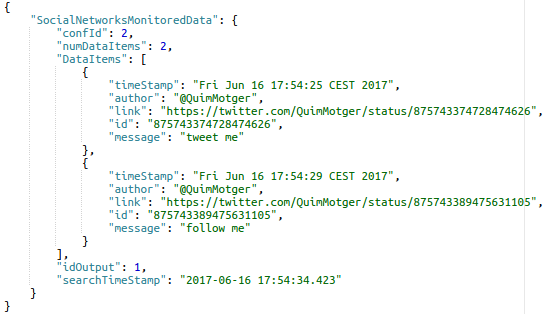
\includegraphics[width=14cm]{Figures/tfg1}
\decoRule
\caption{Primer enviament de dades del monitor de Twitter a Kafka}
\label{fig:tfg1}
\end{figure} 

\begin{figure}[H]
\centering
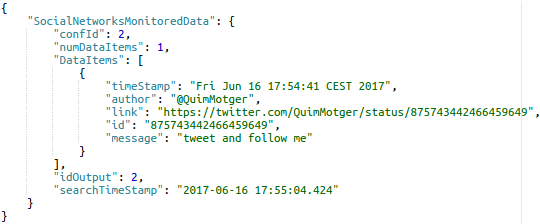
\includegraphics[width=14cm]{Figures/tfg2}
\decoRule
\caption{Segon enviament de dades del monitor de Twitter a Kafka (abans de la reconfiguració)}
\label{fig:tfg2}
\end{figure} 

En aquest punt saltem al 3r enviament de dades, representat a la figura ~\ref{fig:tfg3}. En aquest cas veiem que les dades s'han enviat exactament a \textit{2017-06-16 17:56:05.489}. Si ens fixem, la diferència ha estat d'aproximadament 60 segons exacta respecte al darrer enviament. Aquest comportament és l'esperat i l'explicació és relativament senzilla: quan es produeix una reconfiguració del \textit{timeslot}, aquesta es produeix durant un cicle de monitoratge del monitor. Això vol dir que el cicle actual es "trenca", i per tant al desenvolupar la \textit{tool} del monitor hem de decidir com actuar. En aquest cas, s'ha optat per iniciar un nou temporitzador amb el nou \textit{timeslot}, i un cop completat el nou cicle, s'envien totes les dades acumulades fins al moment. Podríem haver optat per altres opcions, com p.e. enviar totes les dades acumulades fins al moment i començar a partir d'allà un nou cicle; o simplement actualitzar la durada del cicle en procés i fer que aquesta es rebés amb el nou \textit{timeslot} actualitzat. Al tractar-se d'un punt que admet diverses consideracions, i ja que l'arquitectura dona llibertat al programador per decidir com actuar, no ho considerarem un aspecte a tenir en compte, i ens centrarem en la versió que s'ha implementat per aquest projecte.\\

\begin{figure}[H]
\centering
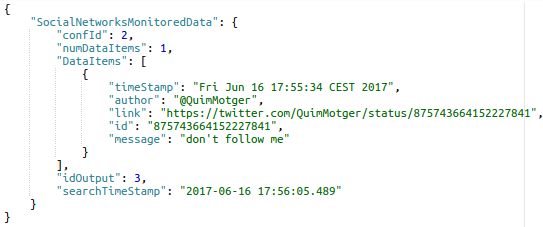
\includegraphics[width=11cm]{Figures/tfg3}
\decoRule
\caption{Tercer enviament de dades del monitor de Twitter a Kafka (després de la reconfiguració)}
\label{fig:tfg3}
\end{figure} 

Per aquesta raó, tot i que podem observar una reconfiguració, veiem que encara no és estable, degut a aquest comportament. Però si observem el següent enviament de dades a la figura ~\ref{fig:tfg4} podem veure com efectivament s'ha actualitzat el \textit{timeslot} amb el valor 50, ja que si comparem el \textit{timestamp} anterior amb el nou, \textit{2017-06-16 17:56:55.489}, veiem que passen exactament 50 segons respecte el 3r enviament. En aquest cas, addicionalment, es mostra un exemple d'enviament de dades buit (és a dir, no s'han trobat tuits que satisfacin els paràmetres de cerca). \\

\begin{figure}[H]
\centering
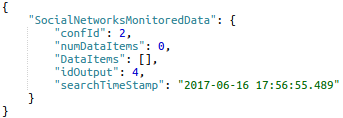
\includegraphics[width=8cm]{Figures/tfg4}
\decoRule
\caption{Quart enviament de dades del monitor de Twitter a Kafka (configuració estable)}
\label{fig:tfg4}
\end{figure} 

Per tant, tal i com hem pogut comprovar, la reconfiguració del monitor de Twitter es produeix satisfactòriament a partir del disparador implementat al \textit{dashboard} que, gràcies al sistema de models, processa i executa a través del sistema d'adaptabilitat, i més tard del de monitoratge, la reconfiguració d'acord amb els criteris definits per aquest modelatge. Aquest, per suposat, es tracta d'un cas bàsic per validar la funcionalitat del nostre sistema. Amb el disseny i implementació d'aquests components, i amb aquest cas d'ús, queda demostrat que el sistema funciona i permet reconfigurar de forma automatitzada processos de monitoratge actius. El potencial de validació de nous casos d'ús, modificacions més complexes, etc., són modificacions que, tot i que queden fora de l'abast d'aquest projecte, són futures tasques sobre les quals aquest desenvolupament suposa una base teòrica i pràctica molt potent sobre la qual treballar.